\section{主観評価におけるアプリケーション開発}
先行研究\cite{cf:kayama}で著者らは,遅延聴覚フィードバックが発話に与える影響について,主観評価実験を行った.
主観評価実験とは,耳介付近に伝達された音に一定の遅延を発生させて外耳道に出力する装置を装着した被験者が,
発話時の違和感を主観的に評価するという内容の調査である.
本節では,開発したアプリケーションの概要を説明し,これを主観評価実験で利用することを想定する.
このアプリケーションにより,データ入力ミスのリスクが減少し,
実験者の負担が軽減されることで,より効率的に多くの実験を実施し,結果を分析することが可能になる.
アプリケーションの外観を図\ref{fig:2_userInterface}に示す.
\begin{figure}[tbp]
  \centering
  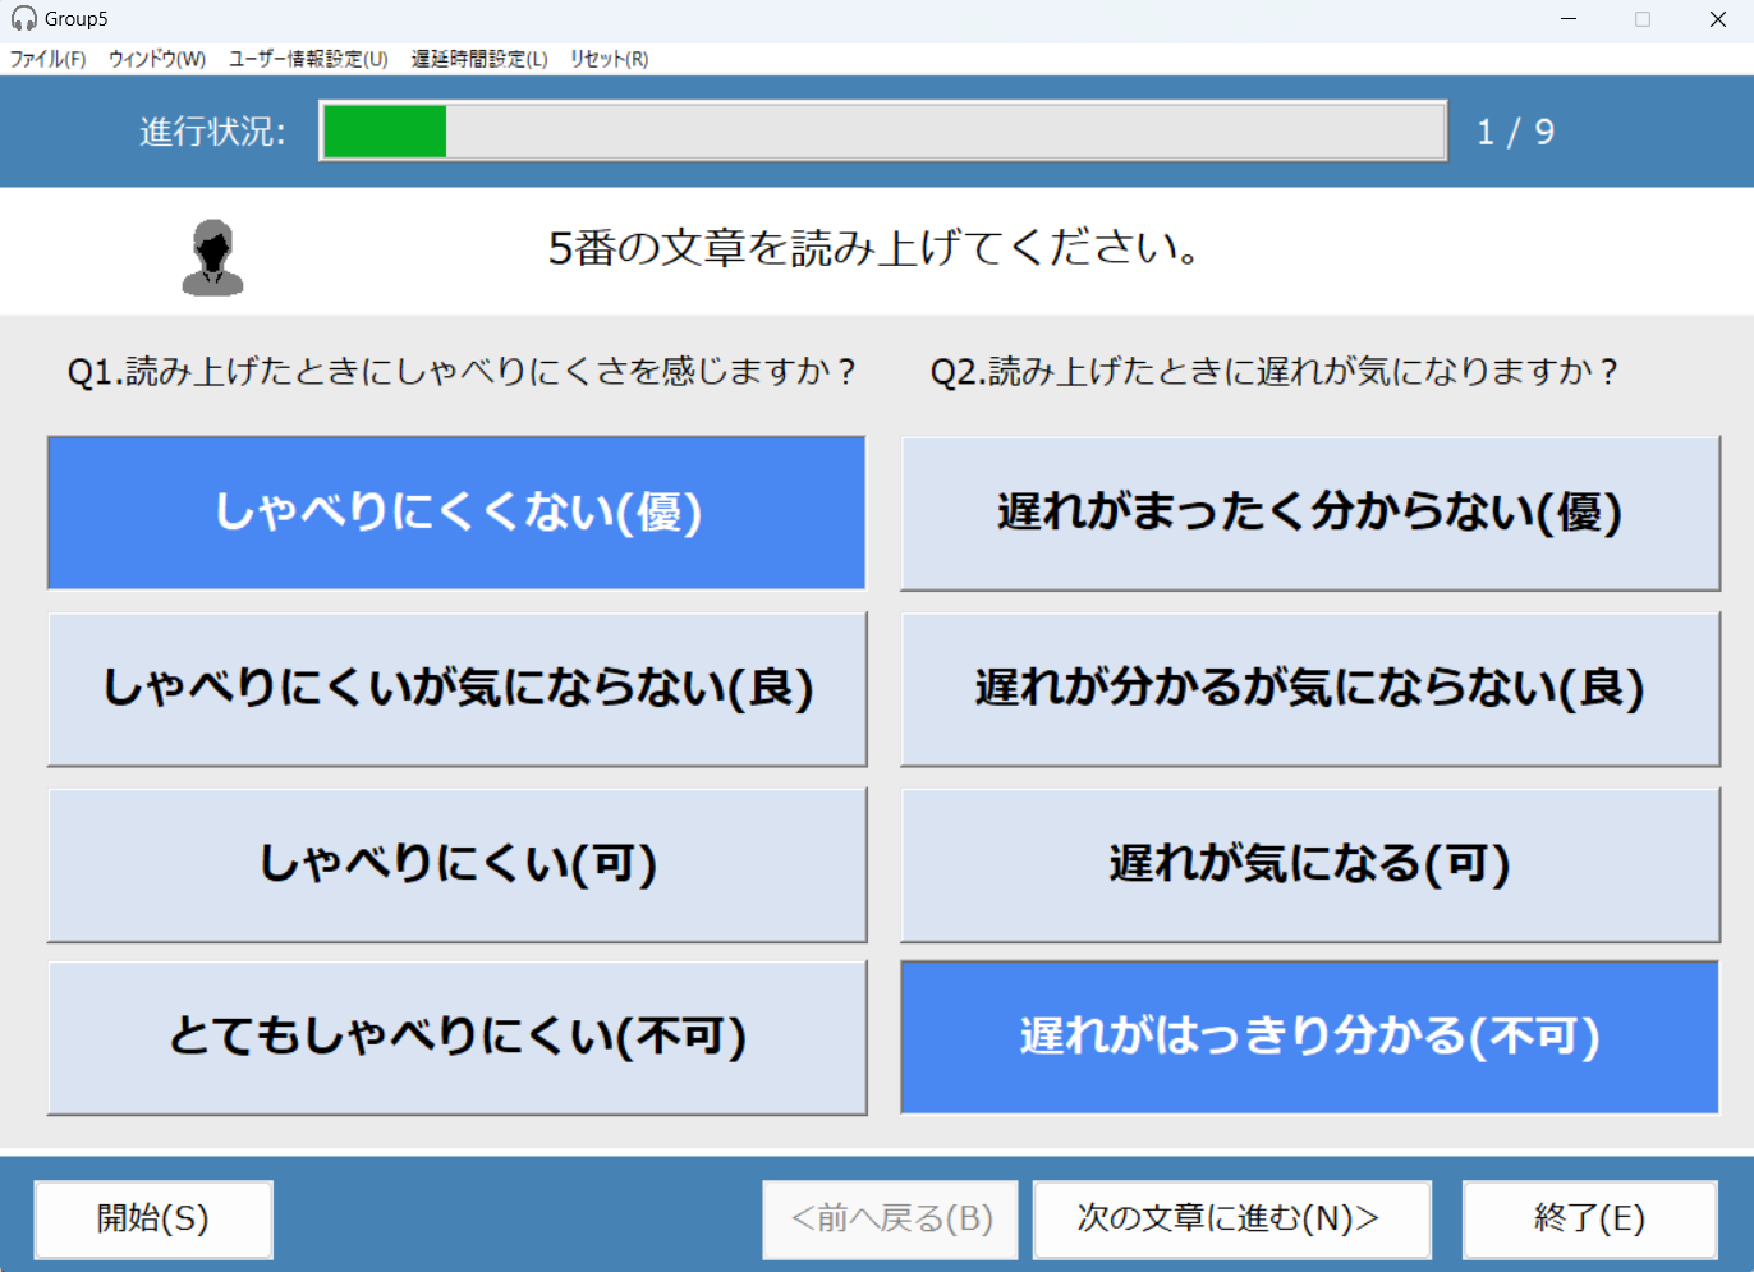
\includegraphics[scale=0.22]{figures/Syukann/app_2.pdf}
  \caption{調査中の画面}
  \label{fig:2_userInterface}
\end{figure}